\chapter{Limits}

The asymptotic behavior we see in rational functions suggests that we need to 
expand our vocabulary of function characteristics. We examined vertical 
asymptotes and end behavior through graphs and tables, and discussed them in 
English. The language of limits enables us to discuss these attributes 
mathematically and with greater efficiency. 

Let's revisit an example from the previous chapter. This function has a hole 
at $ x = 1 $, a vertical asymptote at $ x = 3 $, and a horizontal asymptote of 
$ y = 1 $.

$$ f(x) = \frac{x^2 - 3x + 2}{x^2 - 4x + 3} = \frac{(x-1)(x-2)}{(x-1)(x-3)} $$

\begin{figure}[htbp]
  \centering
  \begin{tikzpicture}
    \begin{axis}[
	  xmin=-5, xmax=5,
	  ymin=-5, ymax=5,
      axis lines = middle,
      xlabel = \(x\),
      ylabel = \(f(x)\),
      restrict y to domain = -10:10,
      samples = 100,
    ]
    \addplot [blue, smooth] {(x - 2)/(x - 3)};
    \draw[dashed] (axis cs: 3,-5) -- (axis cs: 3,5);
    \draw[dashed] (axis cs: -5,1) -- (axis cs: 5,1);
    \end{axis}
  \end{tikzpicture}
  \caption{Graph of \( f(x) = \frac{x^2 - 3x + 2}{x^2 - 4x + 3} \) with 
  asymptotes}
\end{figure}

First, consider the vertical asymptote. We see that the graph goes down as it 
hugs the left side of the vertical asymptote, and goes up as it hugs the right 
side. We can describe these behaviors as the left- and right-hand limits, 
respectively. We say that the left-hand limit of $ f $ at $ x = 3 $ is 
negative infinity. Another way of communicating this is to say that as $ x $ 
approaches $ 3 $ from the left, the function approaches negative infinity. 
Symbolically, we summarize this as 
$$ \lim_{x \rightarrow 3^-} f(x) = -\infty $$

The little negative sign in $x \rightarrow 3^-$ indicates we are approaching 
$x = 3$ from the left (the negative side of the axis). 

Similarly, the right-hand limit of $ f $ at $ x = 3 $ is positive infinity. In 
other words, as $ x $ approaches $ 3 $ from the right, the function approaches 
positive infinity. Symbolically, we write 
$$ \lim_{x \rightarrow 3^+} f(x) = \infty $$

This time, the little $^+$ indicates we are approaching the $x$-value from the 
right (positive) side of the axis. 

The limit of a function at a particular $ x $-value is the $ y $-value that the 
function approaches as it approaches the given $ x $-value. In the previous 
example, we could only specify the left- and right-hand limits, because they were 
different. In cases where the left- and right-hand limits are equal, we can say 
that the function has a limit there. The hole in our function $ f $ is one such 
value. We see that as we approach the hole from both the left and right, the 
function takes on values near $\frac{1}{2}$. This is more apparent numerically:


\begin{center}
\begin{tabular}{ |c|c|c|c|c|c|c|c| } 
 \hline
 x & 0.9 & 0.99 & 0.999 & 1 & 1.001 & 1.01 & 1.1 \\ 
 \hline
 f(x) & 0.5238 & 0.5025 & 0.5003 & undefined & 0.4998 & 0.4975 & 0.4737 \\ 
 \hline
\end{tabular}
\end{center}

We can also see this by zooming in on the graph (see figure \ref{holezoom}):

\begin{figure}[htbp]
\begin{subfigure}{0.5\textwidth}
\centering
    \begin{tikzpicture}
	\begin{axis}[width = 1\textwidth, xmin = 0.5, xmax = 1.5, axis lines = 
	center, xlabel = $x$, x label style = {anchor = north}, ylabel = $f(x)$, 
	y label style = {at={(axis description cs:-0.1,1.2)}, anchor = north}]
        \addplot[blue, thick, domain = 0.5:0.999]{(x^2 - 3*x + 2)/(x^2 - 4*x 
        + 3)};
        \addplot[blue, thick, domain = 1.001:1.5]{(x^2 - 3*x + 2)/(x^2 - 4*x 
        + 3)};
        \addplot[mark = o, blue]coordinates{(1, 0.5)};
        \end{axis}
    \end{tikzpicture}
    \end{subfigure}
    \begin{subfigure}{0.5\textwidth}
\centering
    \begin{tikzpicture}
	\begin{axis}[width = 1\textwidth, xmin = 0.9, xmax = 1.1, axis lines = 
	center, xlabel = $x$, x label style = {at={(axis description cs:1.1,0)}, 
	anchor = north}, ylabel = $f(x)$, y label style = {at={(axis description 
	cs:-0.1,1.2)}, anchor = north}]
        \addplot[blue, thick, domain = 0.9:0.9999]{(x^2 - 3*x + 2)/(x^2 - 4*x 
        + 3)};
        \addplot[blue, thick, domain = 1.0001:1.1]{(x^2 - 3*x + 2)/(x^2 - 4*x 
        + 3)};
        \addplot[mark = o, blue]coordinates{(1, 0.5)};
        \end{axis}
    \end{tikzpicture}
    \end{subfigure}
    \label{holezoom}
    \caption{Two graphs of $f(x) = \frac{x^2 - 3x + 2}{x^2 - 4x + 3}$ zoomed 
    in about $x = 1$}
    \end{figure}

The left-hand and right-hand limits of $ f $ at $ 1 $ are both $\frac{1}{2}$. Since 
they are equal, we can also say that the limit of $ f $ at $ 1 $ is $\frac{1}{2}$. 
This allows us to efficiently discuss the behavior of $ f $ at $ 1 $, even though 
the function is not defined there, as substituting $ 1 $ into the function gives 
division by zero.

$$ \lim_{x \rightarrow 1^-} f(x) = \lim_{x \rightarrow 1^+} f(x) = \lim_{x 
\rightarrow 1} f(x) = \frac{1}{2} $$

We can also talk about limits at $x$-values where nothing weird is happening (that 
is, no hole or vertical asymptote). For example, as $x$ approaches $4$ from the left 
and right, $y$ approaches $2$.

\begin{center}
\begin{tabular}{ |c|c|c|c|c|c|c|c| } 
 \hline
 x & 3.9 & 3.99 & 3.999 & 4 & 4.001 & 4.01 & 4.1 \\ 
 \hline
 f(x) & 2.1111 & 2.0101 & 2.0010 & 2 & 1.9990 & 1.9901 & 1.9091 \\ 
 \hline
\end{tabular}
\end{center}

In this case, since nothing weird is happening, the limit is equal to the function 
value. This is an example of continuity, which we will discuss in more detail in 
the next chapter. By contrast, at the vertical asymptote $ x = 1 $, since the left- 
and right-hand limits are not equal, we say the function does not have a limit, or 
the limit does not exist.

Finally, let's consider the horizontal asymptote of $f$. The graph hugs the line 
$y = 1$ as $x$ goes far to the left and far to the right. We say that as $x$ 
approaches negative infinity, $f$ approaches $1$; likewise, that as $x$ 
approaches positive infinity, $f$ approaches $1$. We write these symbolically as 
$\lim_{x \rightarrow -\infty} f(x) = 1$ and $\lim_{x \rightarrow \infty} f(x) = 1$. 

\begin{Exercise}[title=Limits Practice 1, label=limits1]
  Determine the left- and right-hand limits of the function as $x$ approaches the 
  given values. At $x$-values where the limit exists, determine it.
  \Question{$p(x) = \frac{x + 3}{x^2 + 9x + 18}, x = -6, -5, -3, \infty$}
  \vspace{40mm}
\end{Exercise}
\begin{Answer}[ref=limits1] 
	$$ \lim_{x \rightarrow -6^-} p(x) = -\infty, \lim_{x \rightarrow -6^+} p(x) = \infty $$
	$$ \lim_{x \rightarrow -5^-} p(x) = \lim_{x \rightarrow -5^+} p(x) = \lim_{x \rightarrow -5} p(x) = 1 $$
	$$ \lim_{x \rightarrow -3^-} p(x) = \lim_{x \rightarrow -3^+} p(x) = \lim_{x \rightarrow -3} p(x) = \frac{1}{3} $$
	$$ \lim_{x \rightarrow \infty} p(x) = 0 \text{ called simply a limit, although it is a left-hand limit} $$
\end{Answer}

We have seen two weird behaviors of rational functions at certain $x$-values: holes 
and vertical asymptotes. Now, we will examine another type of weird behavior: jumps. 
This is a characteristic of some piecewise-defined functions. In piecewise-defined 
functions, the domain is divided into two or more pieces, and a different 
expression is used to give the y-value depending on which piece contains the $x$-
value. One common piecewise-defined function is the floor function (shown in 
figure \ref{fig:floor}), sometimes denoted $\lfloor x \rfloor$. The standard 
floor function rounds any real number down to the nearest integer. So, for a 
price quoted in dollars and cents, the floor would just be the number of 
dollars.

\begin{figure}[htbp]
  \centering
	\begin{tikzpicture}
	\begin{axis}[
	    xmin=-5, xmax=5,
	    ymin=-5, ymax=5,
	    axis lines=middle,
	    xlabel={$x$},
	    ylabel={$y$},
	]
	\addplot[domain=-5:5, samples=500, blue] {floor(x)};
	\end{axis}
	\end{tikzpicture}
  \caption{Graph of \( y = \lfloor x \rfloor \)}
  \label{fig:floor}
\end{figure}	

When $x$ is exactly $1$, the function value is $1$: the number of dollars in a 
price of \$1.00. When $x$ is any number greater than $1$ but less than $2$, the 
function value is still $1$. Also, $ \lfloor 1.01 \rfloor, \lfloor 1.5 \rfloor, 
\text{and} \lfloor 1.99999 \rfloor$ are all $1$. As we continue to look to the 
right, once $x$ equals exactly $2$, $h$ jumps up to the value $2$. So, 
$ \lim_{x \rightarrow 2^-} \lfloor x \rfloor = 1 $, while 
$ \lim_{x \rightarrow 2^+} \lfloor x \rfloor = 2 $.

Besides rational and piecewise defined functions, there are other functions with 
interesting limits. Consider the standard exponential function, $y = e^x$ 
(shown in figure \ref{fig:exponent}).

\begin{figure}[htbp]
  \centering
	\begin{tikzpicture}
	\begin{axis}[
	    xmin=-5, xmax=5,
	    ymin=-0, ymax=10,
	    axis lines=middle,
	    xlabel={$x$},
	    ylabel={$y$},
	]
	\addplot[domain=-5:5, samples=500, blue] {exp(x)};
	\end{axis}
	\end{tikzpicture}
  \caption{Graph of \( y = e^x \)}
  \label{fig:exponent}
\end{figure}	

As $x$ increases, $y$ increases without bound; that is, $\lim_{x \rightarrow 
\infty} e^x = \infty$. However, looking far to the left, we see that $y$ hugs the 
$x$-axis. This is because raising $e$ to a large negative exponent is the same as 
$1$ divided by $e$ raised to a large positive exponent; that is, $1$ divided by a 
very large number, which yields a very small positive number. In limit notation, 
$\lim_{x \rightarrow -\infty} e^x = 0$. This example illustrates that horizontal 
asymptotes need not model end behavior in both directions. Note that this reasoning 
holds for $y = b^x$ for any $b > 1$, so all such functions have the same horizontal 
asymptote, $y = 0$.

We know that the natural logarithm function, $y = \text{ln } x$, is the inverse of 
$y = e^x$. Since inverse functions swap the role of $x$ and $y$, it stands to 
reason that a horizontal asymptote in one function corresponds with a vertical 
asymptote in the other function, and that is indeed the case (see figure 
\ref{fig:log}).

\begin{figure}[htbp]
  \centering
	\begin{tikzpicture}
	\begin{axis}[
	    xmin=0, xmax=10,
	    ymin=-5, ymax=5,
	    axis lines=middle,
	    xlabel={$x$},
	    ylabel={$y$},
	]
	\addplot[domain=0.001:10, samples=500, blue] {ln(x)};
	\end{axis}
	\end{tikzpicture}
  \caption{Graph of \( y = \text{ln } x \)}
  \label{fig:log}
\end{figure}	

An untransformed logarithm function is defined only for positive inputs. That is 
because it is not possible to find an exponent of a positive number that will 
yield a negative or zero result. What type of exponent on a positive number yields 
a number near zero? That would be a large-magnitude negative number. So, on the 
logarithm graph, large negative $y$-values correspond with $x$-values only slightly 
greater than zero. So, $\text{ln } x$ (and $\text{log}_2 x$, and indeed 
$\text{log}_b x$ for any $b > 1$) approaches negative infinity as $x$ approaches 
$0$ from the right. There is no left-hand limit at $0$, however. In limit notation, 
$\lim_{x \rightarrow 0^+} \text{ln } x = -\infty$.

\begin{Exercise}[title=Limits Practice 2, label=limits2]
  State the asymptotes of the following transformed exponential and logarithmic 
  functions. Give the limit statement which describes the behavior of the function 
  along the asymptote.
  \Question{$y = 3^x + 1$}
  \Question{$y = \text{log}_2 (x-4)$}
  \Question{$y = 2^{1-x}$}
  \Question{$y = \text{log}_{10} (-2x)$}
  \vspace{40mm}
\end{Exercise}
\begin{Answer}[ref=limits2] 
	$$ \lim_{x \rightarrow -\infty} 3^x + 1 = 1; \lim_{x \rightarrow 4^+} 
	\text{log}_2 (x-4) = -\infty; \lim_{x \rightarrow \infty} 2^{1-x} = 0; \lim_{x 
	\rightarrow 0^-} \text{log}_{10} (-2x) = -\infty $$
\end{Answer}

We next consider two functions that each have two horizontal asymptotes. These two 
seemingly obscure functions are quite important in data science.

\begin{figure}[htbp]
  \centering
  \begin{tikzpicture}
    \begin{axis}[
        xmin=-10, xmax=10,
        ymin=-2, ymax=2,
        axis lines=middle,
        xlabel={$x$},
        ylabel={$y$},
        xtick={-10,-5,...,10},
        ytick={-2,-1,...,2},
    ]
    \addplot[domain=-10:10, samples=200, blue] {rad(atan(x))};
    \draw[dashed] (axis cs:-10,1.5708) -- (axis cs:10,1.5708);
    \draw[dashed] (axis cs:-10,-1.5708) -- (axis cs:10,-1.5708);
    \end{axis}
  \end{tikzpicture}
  \caption{Graph of \(y = \arctan x\)}
\end{figure}

We know that the arctangent, or inverse tangent, function is the inverse of the 
piece of the tangent function which passes through the origin. The vertical 
asymptotes bounding this piece become horizontal asymptotes when the function is 
inverted.

Here are the equation and graph of the logistic function:

\begin{figure}[htbp]
  \centering
  \begin{tikzpicture}
    \begin{axis}[
        xmin=-10, xmax=10,
        ymin=0, ymax=1,
        axis lines=middle,
        xlabel={$x$},
        ylabel={$y$},
        xtick={-10,-5,...,10},
        ytick={0,0.5,1},
    ]
    \addplot[domain=-10:10, samples=200, blue] {1/(1+exp(-x))};
    \draw[dashed] (axis cs:-10,1) -- (axis cs:10,1);
    \draw[dashed] (axis cs:-10,0) -- (axis cs:10,0);
    \end{axis}
  \end{tikzpicture}
  \caption{Graph of the logistic function, $ y = \frac{1}{1 + e^{-x}} $}
\end{figure}

%\begin{figure}[htbp]
%  \centering
%  \begin{tikzpicture}
%    \begin{axis}[
%      axis lines = middle,
%      xlabel = \(x\),
%      ylabel = \( \frac{1}{1 + e^{-x}} \),
%      restrict y to domain = -5:5,
%      samples = 100,
%      xmin = -5, xmax = 5, ymin = 0, ymax = 1.1,
%    ]
%    \addplot [brown, smooth] {1/(1+exp(-x))};
%    \end{axis}
%  \end{tikzpicture}
%  \caption{Graph of the logistic function, $ y = \frac{1}{1 + e^{-x}} $ }
%\end{figure}

For large magnitude negative values of $x$, the exponential term in the denominator 
becomes a very large positive value. The fraction thus becomes a positive number 
very close to zero. For large magnitude positive values of $x$, that exponential 
term becomes a very small positive number. Adding it to $1$ yields a denominator 
just barely greater than $1$. Dividing $1$ by this number therefore yields a function 
value just barely less than $1$. So, the logistic function yields values between 
$0$ and $1$, though never equaling either of these values exactly. It is precisely 
this characteristic which makes the logistic function so useful.

\begin{Exercise}[title=Limits Practice 3, label=limits3]
Using limit notation, state the limits as x approaches negative and positive 
infinity for the inverse tangent and logistic functions given above.
  \vspace{40mm}
\end{Exercise}
\begin{Answer}[ref=limits3] 
	$ \lim_{x \rightarrow -\infty} \text{tan}^{-1}x = -\frac{\pi}{2}, \lim_{x 
	\rightarrow \infty} \text{tan}^{-1}x = \frac{\pi}{2}; \lim_{x \rightarrow 
	-\infty} \frac{1}{1 + e^{-x}} = 0, \lim_{x \rightarrow \infty} \frac{1}{1 + 
	e^{-x}} = 1 $
\end{Answer}


As seen above, the limit of a function from the left may be different from the 
limit of the function from the right. Additionally, the actual \textit{value} of 
the function may be different from the limit. Consider the piecewise function h(x):

$h(x) = \begin{cases}
    -x^2+3, \text{ if } x < 0\\
    2, x=0\\
    -x+3, \text{ if } x > 0
\end{cases}$

\begin{figure}[htbp]
\centering
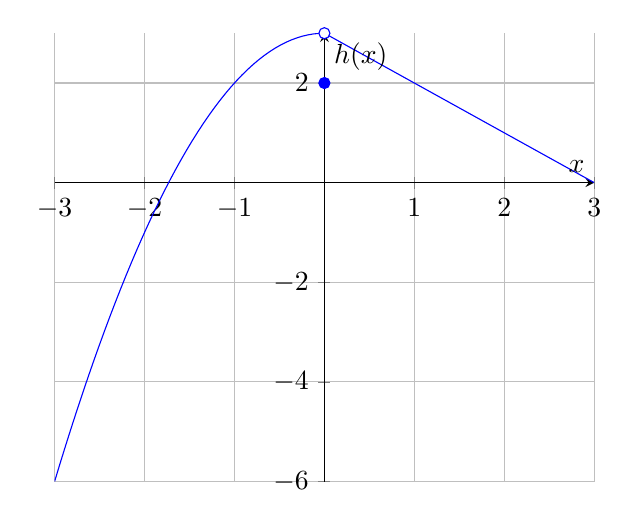
\begin{tikzpicture}
    \begin{axis}
        [grid, axis lines = center, xlabel = \(x\), ylabel=\(h(x)\)]
    \addplot[
    domain=-3:0,
    samples=50,
    color=blue,
    ]
    {-x^2+3};
    \addplot[mark=*,fill=white,draw=blue] coordinates{(0,3)};
    \addplot[mark=*,fill=blue,draw=blue] coordinates{(0,2)};
    \addplot[
    domain=0:3,
    samples=50,
    color=blue,
    ]
    {-x+3};
    \end{axis}
\end{tikzpicture}
\caption{Graph of the piecewise function, $h(x)$}
\end{figure}


From examining the graph, we see that $$\lim_{x\to0_-}h(x) = \lim_{x\to0_+}h(x) = 3$$
However, $h(0) = 2 \neq 3$. So, does this limit exist? It does! The limit of a 
function describes the \textit{behavior} of the function around a particular value, 
not the value of the function itself. In order for a limit to exist, the limits 
from the left and right must be equal to each other, but not necessarily the actual 
value of the function. 

Use the graph of $h(x)$ above and the graphs of $f(x)$ and $g(x)$ below to complete 
the following exercise.
\begin{figure}[htbp]
\centering
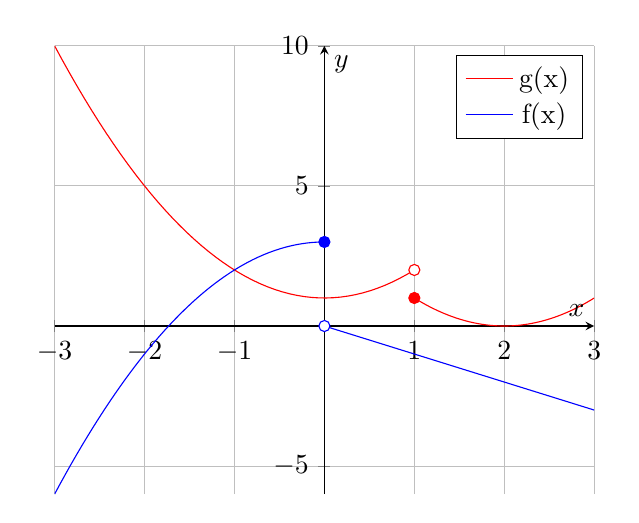
\begin{tikzpicture}
    \begin{axis}[
        grid,
        axis lines = center,
        xlabel = \(x\),
        ylabel = {\(y\)},
        ]
    \addplot [
    domain=-3:1,
    samples=50,
    color=red,
    ]
    {x^2+1};
    \addlegendentry{g(x)};
    \addplot[
    domain=-3:0,
    samples=50,
    color=blue,
    ]
    {-x^2+3};
    \addlegendentry{f(x)};
    \addplot[
    domain=1:3,
    samples=50,
    color=red,
    ]
    {(x-2)^2};
    \addplot[mark=*,fill=red,draw=red] coordinates{(1,1)};
    \addplot[mark=*,fill=white,draw=red] coordinates{(1,2)};
    
    \addplot[mark=*,fill=blue,draw=blue] coordinates{(0,3)};
    \addplot[mark=*, fill=white,draw=blue] coordinates{(0,0)};
    \addplot[
    domain=0:3,
    samples=50,
    color=blue,
    ]
    {-x};
    \end{axis}
\end{tikzpicture}
\caption{Piecewise functions $f(x)$ and $g(x)$}
\end{figure}

\begin{Exercise}[title = Limits Practice 4, label=limits4]
Determine the limit from the left and the right for each function at the given 
value(s). State the limit at that value, if it exists.

\Question $h(x), x=-1, 0, 1$
\Question $f(x), x=-1, 0, 2$
\Question $g(x), x=-2, 0, 1, 2$
\vspace{60mm}
\end{Exercise}
\begin{Answer}[ref=limits4]
    \begin{enumerate}
    \item $\lim_{x\to-1_-}h(x) = 2$ and $\lim_{x\to-1_+}h(x)=2$, therefore the limit exists and $\lim_{x\to-1}h(x)=2$

    $\lim_{x\to0_-}h(x) = 3$ and $\lim_{x\to0_+}h(x)=3$, therefore the limit exists and $\lim_{x\to0}h(x)=3$

    $\lim_{x\to1_-}h(x) = 2$ and $\lim_{x\to1_+}h(x)=2$, therefore the limit exists and $\lim_{x\to1}h(x)=2$
    \item $\lim_{x\to-1_-}f(x)=2$ and $\lim_{x\to-1_+}f(x)=2$, therefore the limit exists and $\lim_{x\to-1}f(x) = 2$.

    $\lim_{x\to0_-}f(x) = 3$ and $\lim_{x\to0_+}f(x) = 0$, and because $\lim_{x\to0_-}f(x) \neq \lim_{x\to0_+}f(x)$, the limit does not exist.

    $\lim_{x\to2_-}f(x) = -2$ and $\lim_{x\to2_+}f(x) = -2$, therefore the limit exists and $\lim_{x\to2}f(x) = -2$.

    \item $\lim_{x\to-2_-}g(x) = -1$ and $\lim_{x\to-2_+}g(x) = -1$, therefore the limit exists and $\lim_{x\to-2}g(x) = -1$.

    $\lim_{x\to0_-}g(x)=1$ and $\lim_{x\to0_+}g(x) = 1$, therefore the limit exists and $\lim_{x\to0}g(x) = 1$

    $\lim_{x\to1_-}g(x) = 2$ and $\lim_{x\to0_+}g(x) = 1$, and because $\lim_{x\to1_-}g(x) = 2 \neq \lim_{x\to0_+}g(x)$, the limit does not exist.

    $\lim_{x\to2_-}g(x) = 0$ and $\lim_{x\to2_+}g(x) = 0$, therefore the limit exists and $\lim_{x\to2}g(x) = 0$
\end{enumerate}
\end{Answer}

\section{Continuity}
A note about continuity:

In order to be able to talk more about limits and know when we can apply certain 
rules and theorems, we first must discuss continuity. A function is continuous if 
there are no "jumps" or "gaps" in the graph of the function. For example, the 
function $f(x) = x^2$ is continuous for all real values of x. On the other hand, 
the function $g(x) = tan(x)$ has many discontinuities, including at $x=\frac{\pi}
{2}$. Let's examine the graph of each of these functions:


\begin{figure}[htbp]
\centering
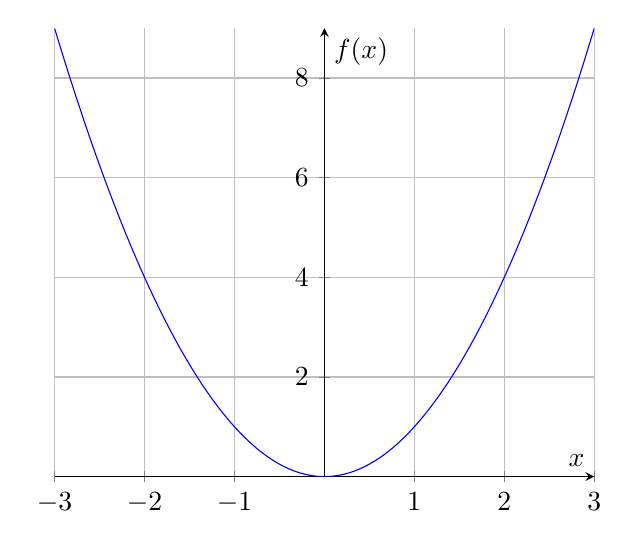
\begin{tikzpicture}
    \begin{axis}[
        grid,
        axis lines = center,
        xlabel = \(x\),
        ylabel = {\(f(x)\)},
        ]
    \addplot [
    domain=-3:3,
    samples=100,
    color=blue,
    ]
    {x^2};
    \end{axis}
\end{tikzpicture}
\caption{Graph of $f(x)=x^2$}
\end{figure}
If you wanted, you could trace your finger along the graph of f(x) from $x=-3$ to 
$x=3$ without ever picking up your finger. This means the function is continuous in 
the domain from $-3 \leq x \leq 3$. In this case, the domain of continuity 
\textit{includes} the end points ($x=3$ and $x=-3$). This is called a closed 
interval. In other cases, the function will be continuous right up to, but not 
including, the endpoints, as with the domains of continuity for our other example, 
$g(x) = \tan{x}$. This is called an open interval. Let's learn more about intervals 
of continuity by examining $g(x) = \tan{x}$.

\begin{figure}[htbp]
\centering
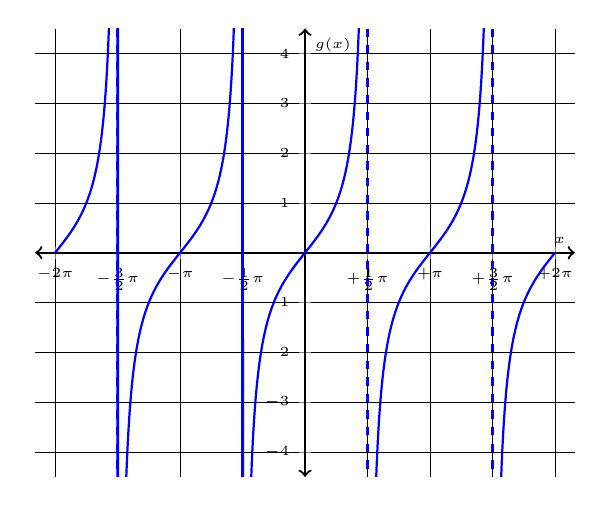
\begin{tikzpicture}
	\begin{axis}[
			axis lines=middle,
			axis line style={thick,<->},
			xmin=-2*pi-0.5,xmax=2*pi+0.5,ymin=-4.5,ymax=4.5,
			ytick={-4,-3,-2,-1,1,2,3,4},
			xtick={-2*pi,-1.5*pi,-pi,-0.5*pi,0,0.5*pi,pi,1.5*pi,2*pi},
			xticklabels={$-2\pi$,$-\frac{3}{2}\pi$,$-\pi$,$-\frac{1}{2}\pi$,$0$,
			$+\frac{1}{2}\pi$,$+\pi$,$+\frac{3}{2}\pi$,$+2\pi$},
			tick label style={font=\tiny},
			grid=major,
			major grid style={very thin,black},
			every axis plot post/.append style={thick},
			label style={font=\tiny},
			xlabel=$x$,
			ylabel=$g(x)$,
			smooth,
					%clip=false,restrict y to domain=-4:4,
					%legend style={
					%font=\tiny,
					%legend cell align=left,
					%legend pos=outer north east,
					%draw=none,
					%empty legend},
					%legend entries={[blue]$y=\sin x$,[green]$y=\cos x$,[brown]$y=\tan x$}
			]
					%\addplot[domain=-2*pi:2*pi,samples=200,blue]{sin(deg(x))};
					%\addplot[domain=-2*pi:2*pi,samples=200,green]{cos(deg(x))};
					%\addplot[domain=-2*pi:2*pi,samples=200,brown]{tan(deg(x))};
	\addplot[domain=-2  *pi:-1.499*pi,samples=200,blue]{tan(deg(x))};
	\addplot[domain=-1.501*pi:-0.499*pi,samples=200,blue]{tan(deg(x))};
	\addplot[domain=-0.501*pi: 0.499*pi,samples=200,blue]{tan(deg(x))};
	\addplot[domain= 0.501*pi: 1.499*pi,samples=200,blue]{tan(deg(x))};
	\addplot[domain= 1.501*pi: 2  *pi,samples=200,blue]{tan(deg(x))};
        \draw[dashed, very thick, blue]  (axis cs: -3*pi/2,-5) -- (axis cs: -3*pi/2,5);
        \draw[dashed, very thick, blue]  (axis cs: -pi/2,-5) -- (axis cs: -pi/2,5);
        \draw[dashed, very thick, blue]  (axis cs: pi/2,-5) -- (axis cs: pi/2,5);
        \draw[dashed, very thick, blue]  (axis cs: 3*pi/2,-5) -- (axis cs: 3*pi/2,5);
	\end{axis}
\end{tikzpicture}
\caption{Graph of $g(x) = \tan{x}$}
\end{figure}

As you can see, if you trace your finger along the graph of the function starting 
at $x=0$, you can continue without lifting your finger to $x=\frac{\pi}{2}$. As you 
approach $x=\frac{\pi}{2}$ from the left, the value of $g(x)$ approaches $\infty$. 
In order to continue tracing the function PAST $x=\frac{\pi}{2}$, you have to lift 
your finger and bring it down to $-\infty$. The function then continues 
continuously again until $x=\frac{3\pi}{2}$. 

In the case of $g(x) = \tan{x}$, the function is continuous on \textit{open 
intervals}, including the open interval $\frac{\pi}{2} < x < \frac{3\pi}{2}$.

There is a shorter way to represent open and closed domain intervals. We can 
represent that $f(x) = x^2$ is continuous on the closed interval $-3 \leq x \leq 3$ 
in the following way: $$x \in \left[3, -3 \right]$$

This reads as "x contained in the domain -3 to 3, inclusive". That is, all the 
values from -3 to 3, including the endpoints. The inclusion of the endpoints is 
implied by the use of \textit{brackets}. For open intervals, we use parentheses to 
communicate that the interval goes up to, but does not include, the endpoints. For 
$g(x) = \tan{x}$, we can use parentheses: 
$$x \in \left(\frac{-3\pi}{2}, \frac{-\pi}{2}\right)$$

because the $g(x) = \tan{x}$ is not continuous at $x=\frac{-3\pi}{2}$ or at 
$x=\frac{-\pi}{2}$.



Formally, a function $f(x)$ is continuous at $x=a$ if $\lim_{x\to a}f(x)$ exists 
\textit{and} $\lim_{x\to a}f(x) = f(a)$. In other words, the limit is equal to the actual 
value of the function. Re-examine the graph of $h(x)$. We have already seen that $
\lim_{x\to 0}h(x)$ exists and is equal to 3. However, $h(0) = 2 \neq \lim_{x\to0}
h(x)$. So $h(x)$ is not continuous at x = 0. Because $-x^2+3$ is evaluable all the 
way to $-\infty$ and $-x+3$ is evaluable all the way to $\infty$, the function 
$h(x)$ is continuous everywhere \textit{except} $x=0$. We can represent this 
mathematically by saying $h(x)$ is continuous on the domain $x \in \left(-\infty, 
0\right)\cup \left(0, \infty\right)$. We use parentheses for $\pm\infty$ because we 
can never actually reach $\infty$. Additionally, the function is continuous up to, 
but not including $0$, and the use of parentheses excludes $x=0$ from the domain of 
continuity.

\subsection{Continuity Practice}
\begin{Exercise}[label = continuity1]
[This problem was originally presented as a calculator-allowed, multiple-
choice question on the 2012 AP Calculus BC exam.] Suppose a function $f$ is 
continuous at $x = 3$. Classify the following statements as always true, 
sometimes true, or never true. Explain your answers. 
\begin{enumerate}
\item $f(3) < \lim_{x \to 3} f(x)$
\item $\lim{x \to 3^+} f(x) \neq \lim_{x \to 3^-} f(x)$
\item $f(3) = \lim_{x \to 3^+} f(x) = \lim_{x \to 3^-} f(x)$
\item The derivative of $f$ at $x = 3$ exists.
\item The derivative of $f$ is positive for $x < 3$ and negative for $x > 3$.
\end{enumerate}
\end{Exercise}

\begin{Answer}[ref = continuity1]
\begin{enumerate}
\item Never true. If a function is continuous at $a$, then $f(a) = \lim_{x \to 
a} f(x)$. 
\item Never true. If a function is continuous at $a$, then $\lim{x \to a^+} 
f(x) = \lim{x \to a^-} f(x)$
\item Always true. This is the definition of continuity.
\item Sometimes true. The derivative of $f$ at $x = 3$ exists for $f(x) = x^2$ 
but not for $f(x) = |x - 3|$.
\item Sometimes true. This statement is true for $f(x) = -(x - 3)^2$ but not 
for $f(x) = 4x$.
\end{enumerate}
\end{Answer}

\begin{Exercise}[title=Limits Practice 5, label=limits5]
State the location of discontinuities (if any) and explain why the function is 
discontinuous at that location:
    \Question $f(x) = \frac{3x^2-8x-3}{x-3}$
    \Question $f(x) = \begin{cases}
    \frac{2}{x^4}, \text{ if } x <\neq 0\\
    2, \text{ if } x=0
    \end{cases}$
    \Question $f(x) = \begin{cases}
        \frac{3x^2-8x-3}{x-3}, \text{ if } x \neq 3\\
        1, \text{ if }, x=3
    \end{cases}$
\end{Exercise}

\begin{Answer}[ref=limits5]
    \begin{enumerate}
    \item $f(x)$ is not defined at $x = 3$. Therefore, it is also discontinuous
     at $x = 3$. As we learn about the continuity of polynomials, we will see 
     why $f(x)$ is continuous everywhere else. 
    \item Here, $f(0)$ is defined, so we need to check if $\lim_{x \to 0}f(x) 
    = f(0)$. The left and right limits as $x$ approaches $0$ are the same 
    ($\infty$), so the limit exists. However, $f(0) = 1 \neq \lim_{x\to 0}f(x)$. 
    Therefore, the function is discontinuous at $x=0$.
    \item In this function, $f(3)$ is defined, so we need to check if the limit 
    equals the function value. The limit of $f(x)$ as $x$ approaches $3$ is: 
    $$\lim_{x \to 3}\frac{3x^2-8x-3}{x-3} = \lim_{x \to 3}
    \frac{(3x+1)(x-3)}{x-3} = \lim_{x \to 3}3x+1 = 10$$
    So the limit exists, but $\lim{x \to 3}f(x) \neq f(3)$, and we see that the 
    function is discontinuous at $x=3$.
	\end{enumerate}
\end{Answer}

\begin{Exercise}[label=limits6]
	The graph of a function, $h(x)$, is shown. Classify each of the following 
	statements as true or false and explain your answer. 
	\\
	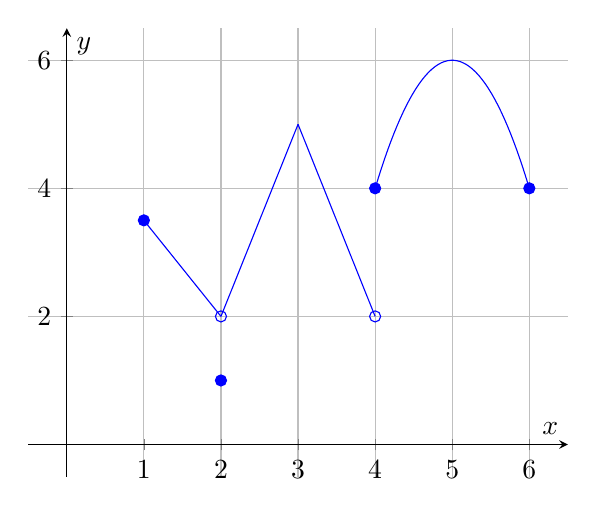
\begin{tikzpicture}
		\begin{axis}[xmin=-0.5, xmax=6.5, ymin=-0.5, ymax=6.5, axis lines = center, xlabel=$x$, ylabel=$y$, grid=major]
		\addplot[blue, mark=*, only marks] coordinates {(1,3.5) (2,1) (4,4) (6,4)};
		\addplot[blue, mark=o, only marks] coordinates {(2,2) (4,2)};
		\addplot[blue, samples=50, domain=1:2]{-1.5*x+5};
		\addplot[blue, samples=50, domain=2:3]{3*x-4};
		\addplot[blue, samples=50, domain=3:4]{-3*x+14};
		\addplot[blue, samples=50, domain=4:6]{-2*(x-5)^2+6};
		\end{axis}
	\end{tikzpicture}
	\begin{enumerate}
	\item $\lim_{x\to2} h(x)$ exists
	\item $\lim_{x \to 3} h(x)$ does not exist
	\item $\lim_{x \to 4} h(x)$ exists
	\item $h(x)$ is continuous at $x=5$
	\item $h(x)$ is not continuous at $x=4$
	\item $\lim_{x \to 2} h(x) = h(2)$
	\end{enumerate}
\end{Exercise}

\begin{Answer}[ref=limits6]
	\begin{enumerate}
	\item True, $h(x)$ approaches 2 from the left and right, therefore the limit 
	exists
	\item False, $h(x)$ approaches 5 from the left and right, therefore the limit 
	exists
	\item False, $h(x)$ approaches 2 from the left and 4 from the right, therefore 
	the limit does not exist
	\item True, $\lim_{x \to 5}h(x) = h(5)$, therefore $h(x)$ is continuous at $x=5$
	\item True, $\lim_{x \to 4}h(x)$ does not exist, therefore $h(x)$ is 
	discontinuous at $x=4$
	\item False, $h(2) = 1 \neq 2 = \lim_{x \to 2}h(x)$
	\end{enumerate}
\end{Answer}

\section{Limits Rules}
There are some mathematical properties of limits which allow us to determine the 
limit of complex functions without seeing a graph or using a calculator to generate 
a table. 

The following laws are true given that \textit{c} is a constant, $\lim_{x\to a} 
f(x) $ exists, and $\lim_{x\to a} g(x) $ exists.

\begin{enumerate}
    \item Sum Law $\lim_{x\to a} \left[f(x) + g(x) \right] = lim_{x\to a} f(x) 
    + lim_{x\to a} g(x)$
    \item Difference Law $\lim_{x\to a} \left[f(x) - g(x) \right] = 
    lim_{x\to a} f(x) - \lim_{x\to a} g(x)$
    \item Constant Multiple Law $\lim_{x\to a} \left[\textit{c}f(x) \right] = 
    \textit{c} \cdot \lim_{x\to a} f(x) $
    \item Product Law $\lim_{x\to a} \left[f(x)g(x) \right] = lim_{x\to a}f(x) 
    \cdot \lim_{x\to a} g(x)$
    \item Quotient Law $\lim_{x\to a} \frac{f(x)}{g(x)} = \frac{\lim_{x\to a} 
    f(x)}{\lim_{x\to a} g(x)}$ given that $\lim_{x\to a} g(x) \neq 0$
\end{enumerate}
These laws are fairly obvious --- the limit of the sum of two functions is equal to 
the sum of the limits of each function individually. The only tricky one is the 
last: The limit of the quotient of two functions is equal to the quotient of the 
limits if and only if the limit of the function in the denominator does not equal 
zero. This makes sense, as we know dividing by zero yields an undefined result. 

Let's practice applying these laws to evaluate the limits of the functions f(x), 
shown in blue below, and g(x), shown in red below:

$f(x) = \begin{cases}
    -x^2+3, \text{ if } x \leq 0\\
    -x, \text{ if } x > 0
\end{cases}$

$g(x) = \begin{cases}
   x^2+1, \text{ if } x < 1 \\
    (x-2)^2, \text{ if } x \geq 1
\end{cases}$

\begin{figure}[htbp]
\centering
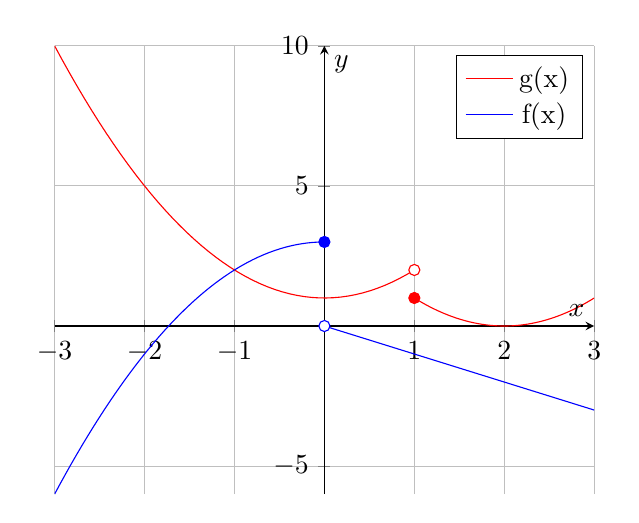
\begin{tikzpicture}
    \begin{axis}[
        grid,
        axis lines = center,
        xlabel = \(x\),
        ylabel = {\(y\)},
        ]
    \addplot [
    domain=-3:1,
    samples=50,
    color=red,
    ]
    {x^2+1};
    \addlegendentry{g(x)};
    \addplot[
    domain=-3:0,
    samples=50,
    color=blue,
    ]
    {-x^2+3};
    \addlegendentry{f(x)};
    \addplot[
    domain=1:3,
    samples=50,
    color=red,
    ]
    {(x-2)^2};
    \addplot[mark=*,fill=red,draw=red] coordinates{(1,1)};
    \addplot[mark=*,fill=white,draw=red] coordinates{(1,2)};
    
    \addplot[mark=*,fill=blue,draw=blue] coordinates{(0,3)};
    \addplot[mark=*, fill=white,draw=blue] coordinates{(0,0)};
    \addplot[
    domain=0:3,
    samples=50,
    color=blue,
    ]
    {-x};
    \end{axis}
\end{tikzpicture}
\caption{Graphs of the piecewise functions $f(x)$ and $g(x)$}
\end{figure}
We can use these laws to evaluate limits involving $f(x)$ and $g(x)$ (shown on the 
graph above). Here are some examples:
Use the graphs of f(x) and g(x) given above to evaluate each limit, if it exists. 
If the limit does not exist, explain why. Two examples are given first:

\textbf{Example 1}: Evaluate $\lim_{x\to0} f(x) \cdot g(x)$

\textbf{Solution 1}: From the Product Law, we know that:
$$\lim_{x\to0} f(x) \cdot g(x) = \lim_{x\to0}f(x) \cdot \lim_{x\to0} g(x)$$

Looking at the graph, we can see that 
$$\lim_{x\to0}g(x) = 1$$ 

and there is a discontinuity in $f(x)$ at $x=0$. Therefore, 
$$\lim_{x\to0}f(x) = \text{undef}$$

Substituting this, we get: 
$$\lim_{x\to0}f(x) \cdot \lim_{x\to0} g(x) = \text{undef} \cdot 1 = \text{undef}$$

Therefore, \textit{the limit does not exist}. 

\textbf{Example 2}: Evaluate $\lim_{x\to2}f(x) - g(x)$

\textbf{Solution 2}: Applying the Difference Law, we see that:

$$\lim_{x\to2}[f(x) - g(x)] = \lim_{x\to2}f(x) - \lim_{x\to2}g(x)$$

Examining the graph, we see that 
$$\lim_{x\to2}f(x) = -2$$ 

and 
$$\lim_{x\to2}g(x) = 0$$

Substituting these values, we get:

$$\lim_{x\to2}f(x) - g(x) = -2 - 0 = -2$$

\begin{Exercise}
    [title = Limits Practice 6, label=limits6]
\begin{enumerate}
    \item $\lim_{x\to-3} \frac{f(x)}{g(x)}$
    \item $\lim_{x\to2}\left[f(x) + 5g(x)\right]$
    \item $\lim_{x\to-1} \frac{3g(x)}{f(x)}$
    \item $\lim_{x\to0}f(x) \cdot 5g(x)$
    \item $\lim_{x\to-1} f(x) - 3g(x) $
\end{enumerate}
\vspace{40mm}
\end{Exercise}
\begin{Answer}
    [ref=limits6]
    \begin{enumerate}
        \item From the quotient law, we know that:
        $$\lim_{x\to3}\frac{f(x)}{g(x)}=\frac{\lim_{x\to3}f(x)}{\lim_{x\to3}g(x)}$$\\
        From the graph, we see that: 
        $$\lim_{x\to3}f(x) = -3$$ \\
        and that:
        $$\lim_{x\to3}g(x) = 1$$ \\
        Substituting these values, we get: 
        $$\lim_{x\to3}\frac{f(x)}{g(x)}=\frac{-3}{1} = -3$$
        \item From the Sum Law, we know that: 
        $$\lim_{x\to2}\left[f(x) + 5g(x)\right]=\lim_{x\to2}f(x) + \lim_{x\to2}5g(x)$$\\
        and applying the Constant Multiple Law, we see that: 
        $$\lim_{x\to2}\left[f(x) + 5g(x)\right]=\lim_{x\to2}f(x) + 5\lim_{x\to2}g(x)$$\\
        Examining the graph of f(x) and g(x), we can determine that 
        $$\lim_{x\to2}f(x) = -2$$ \\
        and 
        $$\lim_{x/to2}g(x) = 0$$\\ 
        Substituting these values, we get: 
        $$\lim_{x\to2}\left[f(x) + 5g(x)\right]=-2 + 5 \cdot 0 = -2$$\\
        \item From the quotient law, we see that: 
        $$\lim_{x\to-1} \frac{3g(x)}{f(x)}=\frac{\lim_{x\to-1}3g(x)}{\lim_{x\to-1}f(x)}$$\\ 
        Applying the Constant Multiple Law, we get: 
        $$\lim_{x\to-1} \left[\frac{3g(x)}{f(x)}\right]=\frac{3\lim_{x\to-1}g(x)}{\lim_{x\to-1}f(x)}$$\\ 
        From the graph, we see that: 
        $$\lim_{x\to-1}f(x) = 2$$\\
        and 
        $$\lim_{x\to-1}g(x) = 2$$\\ 
        Substituting, we get: 
        $$\lim_{x\to-1} \left[\frac{3g(x)}{f(x)}\right]=\frac{3 \cdot 2}{2}=3$$\\
        \item Applying the Product and Constant Multiple Laws, we get: 
        $$\lim_{x\to0}\left[f(x) \cdot 5g(x)\right] = \lim_{x\to0}f(x) \cdot 5 \cdot \lim_{x\to0}g(x)$$\\
        Examining the graphs, we see that $\lim_{x\to0}f(x)$ does not exist and 
        $\lim_{x\to0}g(x) = 1$. Because $\lim_{x\to0}f(x)$ does not exist, 
        $\lim_{x\to0}f(x) \cdot 5 \cdot \lim_{x\to0}g(x)$ also does not exist. 
        \item Applying the Difference and Constant Multiple Laws, we see that: 
        $$\lim_{x\to-1} \left[f(x) - 3g(x)\right] =\lim_{x\to-1}f(x) - 3 \cdot \lim_{x\to-1}g(x)$$ \\
        Examining the graphs, we see that: 
        $$\lim_{x\to-1}f(x) = 2$$\\ 
        and 
        $$\lim_{x\to-1}g(x) = 2$$\\ 
        Substituting, we get that: 
        $$\lim_{x\to-1} \left[f(x) - 3g(x)\right] =2 - 3 \cdot 2 = 2-6 = -4$$\\
    \end{enumerate}
\end{Answer}


Recall that exponents represent repeated multiplication. Therefore, if we apply the 
Product Law multiple times, we obtain the Power Law for limits:
\begin{enumerate}
    \setcounter{enumi}{5}
    \item Power Law $\lim_{x \to \infty} \left[ f(x) \right]^n = \left[ 
    \lim_{x \to \infty} f(x) \right]^n$ where n is a positive integer
\end{enumerate}
There are two special limits that will be useful to us and are intuitively 
obvious, but we won't formally prove here.  
\begin{enumerate}
    \setcounter{enumi}{6}
    \item $\lim_{x\to a} \textit{c} = \textit{c}$
    \item $\lim_{x\to a} x = a$
\end{enumerate}
Combining Law 8 with the Power Law, we find that:
\begin{enumerate}
\setcounter{enumi}{8}
    \item $\lim_{x\to a} x^n = a^n$
\end{enumerate}
And similarly, for square roots:
\begin{enumerate}
    \setcounter{enumi}{9}
    \item $\lim_{x\to a} \sqrt[n]{x} = \sqrt[n]{a}$ (if n is even, we assume $a > 0$)
\end{enumerate}

Direct substitution property: If $f$ is a polynomial or rational function and $a$ 
is in the domain for $f$, then $$\lim_{x \to a}f(x) = f(a)$$

Often, rational functions can be simplified. In an above example, we computed the 
limit by simplifying $f(x) = \frac{3x^2-8x-3}{x-3}$ to the simpler $g(x) = 3x+1$. 
This is a valid strategy because $\frac{3x^2-8x-3}{x-3} = 3x+1$ when $x \neq 3$. 
Remember: a limit describes how a function behaves \textit{as it approaches} $a$, 
not its value/behavior when $x$ \textit{actually equals} $a$. This reveals the 
following useful rule: 
$$\text{If } f(x)=g(x) \text{ when } x \neq a \text{, then } 
\lim_{x \to a}f(x) = \lim_{x \to a}g(x) \text{, provided the limit exists.}$$

\section{Squeeze Theorem}

The Squeeze Theorem states that if $f(x) \leq g(x) \leq h(x)$ when $x$ is near $a$ 
(except at $a$) and $$\lim_{x \to a}f(x)=\lim_{x \to a}h(x) = L$$, then $$\lim_{x 
\to a}g(x) = L$$

In other words, if $g(x)$ is between $f(x)$ and $h(x)$ near $a$, and $f$ and $h$ have the 
same limit, $L$, then the limit of $g$ must also be $L$. 

\textbf{Example}: Let's examine the graph of $g(x) = x^2\sin{\frac{1}{x}}$ and determine $\lim_{x \to 
0}g(x)$:

\begin{figure}[htbp]
\centering
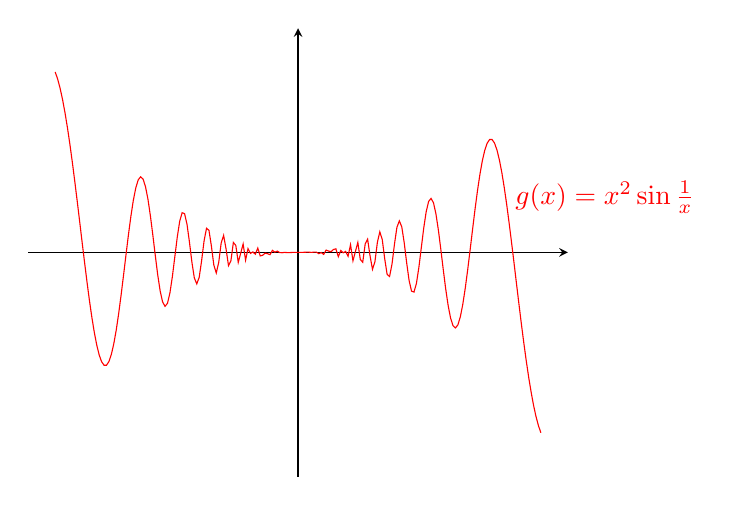
\begin{tikzpicture}
    \begin{axis}[clip=false,
    xmin=-.1, xmax=.1,
    ymin=-.01, ymax=0.01,
    axis lines=middle,
    xtick=\empty,
    ytick=\empty,
    ]
     \addplot[domain=-.09:0.09, red, samples=200]{(x^2)*sin(deg(1/x))}
     node[right, pos=0.92]{$g(x)=x^2\sin{\frac{1}{x}}$}; 
     %\addplot[domain=-.09:0.09, blue, samples=50]{x^2}
     %node[right, pos=0.95]{$g(x)=x^2$};
     %\addplot[domain=-.09:0.09, black, samples=50]{-x^2}
     %node[right, pos=1]{$h(x)=-x^2$};
    \end{axis}
\end{tikzpicture}
\caption{Graph of $g(x) = x^2\sin{\frac{1}{x}}$}
\end{figure}

\textbf{Solution}: Because $\sin{\frac{1}{x}}$ is undefined at $x=0$, we cannot 
compute the limit directly. However, from examining the graph, we can guess 
that $\lim_{x \to 0} g(x) = 0$. Feel free to confirm this with your calculator. 
We need to choose two functions: one that is larger than $g(x)$ near $x = 0$ 
and one that is smaller. Since $|\sin{\frac{1}{x}}|\leq 1$ (when $x \neq 0$), 
then $$|x^2 \sin{\frac{1}{x}}| \leq x^2$$ and $$-x^2 \leq x^2 \sin{\frac{1}{x}} 
\leq x^2$$

Let's confirm this by plotting $f(x)=-x^2$, $g(x)$, and $h(x)=x^2$ on the same 
graph:

\begin{figure}[htbp]
\centering

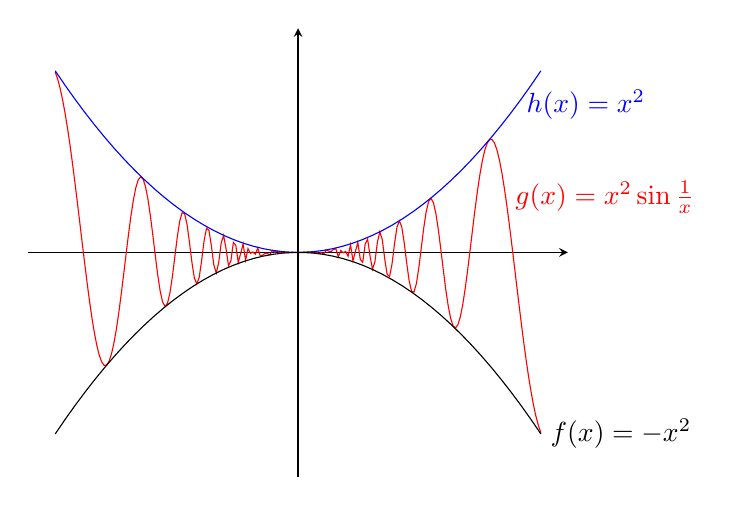
\begin{tikzpicture}
    \begin{axis}[clip=false,
    xmin=-.1, xmax=.1,
    ymin=-.01, ymax=0.01,
    axis lines=middle,
    xtick=\empty,
    ytick=\empty,
    ]
     \addplot[domain=-.09:0.09, red, samples=200]{(x^2)*sin(deg(1/x))}
     node[right, pos=0.92]{$g(x)=x^2\sin{\frac{1}{x}}$}; 
     \addplot[domain=-.09:0.09, blue, samples=50]{x^2}
     node[right, pos=0.95]{$h(x)=x^2$};
     \addplot[domain=-.09:0.09, black, samples=50]{-x^2}
     node[right, pos=1]{$f(x)=-x^2$};
    \end{axis}
\end{tikzpicture}
\caption{Squeeze Theorem example}
\end{figure}

As you can see, when $x$ is near $0$, $f(x) \leq g(x) \leq h(x)$. Because $f(x)$ 
and $h(x)$ are both polynomials, their limits are straightforward: $$\lim_{x \to 
0}-x^2 = 0 \text{ and } \lim_{x \to 0}x^2 = 0$$

Then, by the Squeeze Theorem, we can say that: $$\lim_{x \to 0}x^2\sin{\frac{1}{x}}
=0$$

\subsection{Squeeze Theorem Practice}

\begin{Exercise}
[title=Squeeze Theorem 1, label=squeeze1]
    Use the Squeeze Theorem to show that $\lim_{x \to 0}\sqrt{x^3 + x^2}
    \cos{\frac{1}{x}} = 0$. Illustrate by graphing the functions you define as 
    $f$, $g$, and $h$ on the same plot.
    \vspace{100mm}
\end{Exercise}
\begin{Answer}
    [ref=squeeze1]
    Let $f(x) = -\sqrt{x^3+x^2} \text{ and } h(x) = \sqrt{x^3+x^2}$. Near $0$, 
    $f(x) \leq \sqrt{x^3 + x^2}\cos{\frac{1}{x}} \leq h(x)$. Additionally, 
    $\lim_{x \to 0}f(x) = \lim_{x \to 0}h(x) = 0$. Therefore, by the Squeeze 
    Theorem, we can state that $\lim_{x \to 0}\sqrt{x^3 + x^2}\cos{\frac{1}{x}} 
    = 0$. Plotting all three functions, we can confirm our answer:

  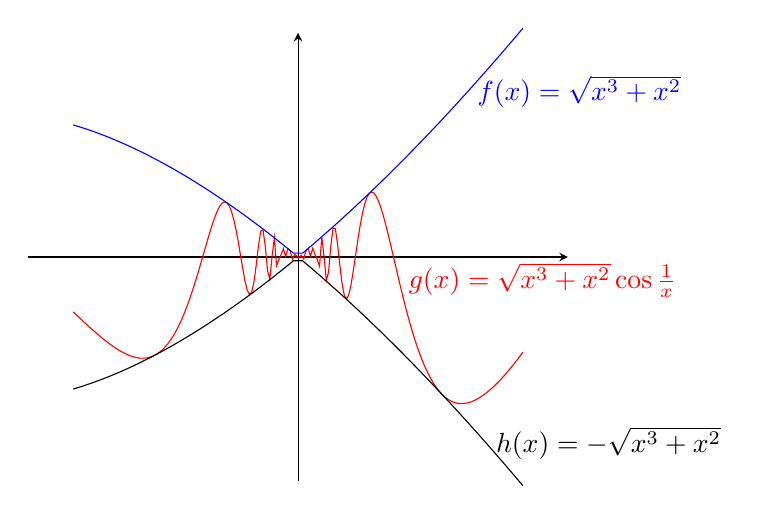
\begin{tikzpicture}
    \begin{axis}[clip=false,
    xmin=-.6, xmax=.6,
    ymin=-.6, ymax=0.6,
    axis lines=middle,
    xtick=\empty,
    ytick=\empty,
    ]
    \addplot[domain=-0.5:0.5, red, samples=200]{sqrt(x^3+x^2)*cos(deg(1/x))}
    node[right, pos=0.83]{$g(x)=\sqrt{x^3+x^2}\cos{\frac{1}{x}}$};
    \addplot[domain=-0.5:0.5, blue, samples=50]{sqrt(x^3+x^2)}
    node[right, pos=0.85]{$f(x)=\sqrt{x^3+x^2}$};
    \addplot[domain=-0.5:0.5, black, samples=50]{-sqrt(x^3+x^2)}
    node[right, pos=0.9]{$h(x) = -\sqrt{x^3+x^2}$};
    \end{axis}
\end{tikzpicture}  
\end{Answer}

\begin{Exercise}
    [title=Squeeze Theorem 2, label=squeeze2]
    If $2x+3 \leq f(x) \leq x^2-2x+7$ for $x \geq 0$, find $\lim_{x \to 2}f(x)$
    \vspace{40mm}
\end{Exercise}
\begin{Answer}
    [ref=squeeze2]
    The question tells us that the function in question, $f(x)$, is between 
    two other functions. $\lim_{x \to 2}2x+3 = 2(2)+3 = 7$ and $\lim_{x \to 2} 
    x^2 - 2x + 7 = 2^2 - 2(2) + 7 = 7$. Since the limits are equal, by Squeeze 
    Theorem we can also know that $\lim_{x \to 2}f(x) = 7$.
\end{Answer}

\begin{Exercise}
    [title= Squeeze Theorem 3, label=squeeze3]
    Prove that $\lim_{x \to 0^+}\sqrt{x}e^{\sin{\frac{\pi}{x}}} = 0$
    \vspace{40mm}
\end{Exercise}

\begin{Answer}
    [ref=squeeze3]
    Note that we can only evaluate the limit from the right, as the domain for this 
    function is $x \geq 0$. Since the range of the sine function is $[-1,1]$, we 
    can state that $$-1 \leq \sin{\frac{\pi}{x}} \leq 1$$ 
    and therefore $$\frac{1}{e} \leq e^{\sin{\frac{\pi}{x}}} \leq e$$. Because 
    we assume the positive root, it is also true that $$\frac{\sqrt{x}}{e} \leq 
    \sqrt{x}e^{\sin{\frac{\pi}{x}}} \leq \sqrt{x}e$$. Taking the limits of the 
    border functions, we see that $$\lim_{x \to 0^+}\frac{\sqrt{x}}{e} = \lim_{x 
    \to 0^+}\sqrt{x}e = 0$$ Therefore, $$\lim_{x \to 0^+}\sqrt{x}e^{\sin{\frac{\pi}
    {x}}}=0$$
\end{Answer}


\section{Intermediate Value Theorem}
When considering functions that are continuous on a closed interval, the 
Intermediate Value Theorem can help us: Given a function, $f(x)$, that is 
continuous on the closed interval $\left[a, b\right]$ and $f(a) \neq f(b)$, 
there is at least one number $c$ such that $f(c) = N$, where $N$ is any number 
between $f(a)$ and $f(b)$. The theorem is illustrated in figures \ref{fig:IVT1} 
and \ref{fig:IVT2}:

\begin{figure}[hbtp]
\centering
\begin{tikzpicture}
    \begin{axis}[
    axis lines = left, 
    xlabel = \(x\), 
    ylabel=\(f(x)\), 
    ymin=0, 
    xtick=\empty,
    ytick=\empty,
    extra y ticks={2.5,6.5, 4.3},
    extra y tick labels={$f(a)$, $f(b)$, $N$},
    extra x ticks = {0.265, 3.75, 3.465},
    extra x tick labels = {$a$, $b$, $c$}
    ]
        \addplot[domain = 0:4, samples =50, color=blue]{(x-1.8)^3-2*(x-1.8)+3};
        \addplot[domain=0:3.75, color=green]{6.5};
        \addplot[samples=50,domain=0:6,green] coordinates {(3.75,0)(3.75,6.5)};
        \addplot[domain = 0:0.265, samples = 50, color=green]{2.5};
        \addplot[samples=50,domain=0:6,green] coordinates {(0.265,0)(0.265, 2.5)};
        \addplot[domain=0:3.465, color=red]{4.3};
        \addplot[domain=0:6, red] coordinates{(3.465,0)(3.465,4.3)};
    \end{axis}
\end{tikzpicture}
\caption{An example where one solution satisfies the Intermediate Value Theorem}
\label{fig:IVT1}
\end{figure}

\begin{figure}[htbp]
\centering
\begin{tikzpicture}
    \begin{axis}[
    axis lines = left, 
    xlabel = \(x\), 
    ylabel=\(f(x)\), 
    ymin=0,
    xtick=\empty,
    ytick=\empty,
    extra y ticks={2.5,6.5, 3.2},
    extra y tick labels={$f(a)$, $f(b)$, $N$},
    extra x ticks = {0.265, 3.75, 0.445, 1.7, 3.25},
    extra x tick labels = {$a$, $b$, $c_1$, $c_2$, $c_3$}
    ]
        \addplot[domain = 0:4, samples =50, color=blue]{(x-1.8)^3-2*(x-1.8)+3};
        \addplot[domain=0:3.75, color=green]{6.5};
        \addplot[samples=50,domain=0:6,green] coordinates {(3.75,0)(3.75,6.5)};
        \addplot[domain = 0:0.265, samples = 50, color=green]{2.5};
        \addplot[samples=50,domain=0:6,green] coordinates {(0.265,0)(0.265, 2.5)};
        \addplot[samples=50, red, domain=0:3.25]{3.2};
        \addplot[samples=50,domain=0:6,red] coordinates {(0.445,0)(0.445, 3.2)};
        \addplot[samples=50,domain=0:6,red] coordinates {(1.7,0)(1.7, 3.2)};
        \addplot[samples=50,domain=0:6,red] coordinates {(3.25,0)(3.25, 3.2)};
    \end{axis}
\end{tikzpicture}
\caption{An example where more than one solution satisfies the Intermediate 
Value Theorem}
\label{fig:IVT2}
\end{figure}

Logically, we can think of the IVT this way: If a function is continuous on a 
closed interval, there are no gaps or breaks. If there are no gaps or breaks, 
then the function must pass through the line $y=N$, since it cannot jump over 
the line. Your graphing calculator uses IVT to find roots of functions: 

\textbf{Example}: Show that there is at least one root of the equation $2x^3 - 
6x^2 + 3x - 1 = 0$ between $x = 2$ and $x = 3$.

\textbf{Solution}: For IVT to apply, we must first check that the function is 
continuous on the closed interval $x \in \left[2, 3\right]$. We define $f(x) = 
2x^2-6x^2+3x-1$, which is continuous everywhere, because it is a polynomial 
function. \textit{For more complex functions, always be sure to check the 
endpoints of an interval, since IVT only applies on closed intervals of 
continuity}. We will take $a = 2$, $b = 3$, and $N = 0$. We find the values of 
$f(x)$ at the endpoints: 

$$f(2) = 2(2)^3 - 6(2)^2 + 3(2) - 1 = 16 - 24 + 6 - 1 = -3$$
$$f(3) = 2(3)^3 - 6(3)^2 + 3(3) - 1 = 54 - 54 + 9 - 1 = 8$$

Therefore, $f(2)<0<f(3)$ and according to IVT, there must exist some $c$ such 
that $f(c) = 0$ and there is a root to the equation in the interval $x \in 
\left(2, 3\right)$.

\begin{Exercise}
    [title=Intermediate Value Theorem Practice, label=IVTPrac]
    Use the IVT to show there is a solution the given equation on the stated 
    interval:\
    \begin{enumerate}
        \item $2x^4+x-12=0 \text{ , } \left(1, 2\right)$
        \item $\ln(x)=3x-4\sqrt{x}\text{ , } \left(2, 3\right)$
        \item $2\sin{x} = 3x^2-2x\text{ , } \left(1, 2\right)$
        \vspace{75mm}
    \end{enumerate}
\end{Exercise}
\begin{Answer}
    [ref=IVTPrac]
    \begin{enumerate}
        \item define $f(x)=2x^4+x-12$, $a=1$, $b=2$, and $N=0$. Calculate 
        $f(a)$ and $f(b)$:
        $$f(1)=-9 \text{ and } f(2)=22$$ \\
        Since $f(x)$ is a polynomial, it is continuous on the interval $x\in
        \left[1, 2\right]$ and we see that $f(a) < 0 < f(b)$. Therefore, there 
        exists some $c \in \left[1, 2\right]$ such that $f(c)=0$.\
        
        \item First, we can rearrange the equation we are considering and 
        define $f(x) = \ln{x} - 3x + 4\sqrt{x}$, and realize we are looking for 
        values where $f(x) = 0$. Both $\ln{x}$ and $\sqrt{x}$ are only continuous 
        for $x > 0$. The interval we are interested in, $x \in \left[2, 
        3\right]$, is in the domain of continuity for both $\ln{x}$ and 
        $\sqrt{x}$. Defining $a = 2$, $b = 3$, and $N = 0$, we find that $f(a) 
        = 0.35 > N > -0.973 = f(b)$. Since $N \in \left[f(b), f(a)\right]$, 
        there must exist some $c$ such that $f(c) = N = 0$ and there is a 
        solution to the equation $\ln{x} = 3x - 4\sqrt{x}$ on the interval $x 
        \in \left(2, 3\right)$.
        
        \item Similar to above, define $f(x) = 2\sin{x} - 3x^2 + 2x$, $a = 1$, 
        $b = 2$, and $N = 0$. Calculate that $f(a) = 0.683$ and $f(b) = -6.181$. 
        Since $f(x)$ is continuous on the interval $ x \in \left[1, 2\right]$ 
        and $f(b) < N < f(a)$, there exists some $c \in \left(1, 2 \right)$ 
        such that $f(c) = 0$. Therefore, there is a solution to $\sin{x} = 
        3x^2 - 2x$ on the interval $ x\in \left(1, 2\right)$.
    \end{enumerate}
\end{Answer}

%Here is a function:
%
%$$f(x) = \frac{x^2}{x} + 1$$
%
%This $f$ is defined for any real number \emph{except 0}. (You can't
%divide anything, including zero, by zero.)
%
%Let's plot $f$:
%
%\begin{tikzpicture}[
%tl/.style = {% tick labels
%    fill=white, inner sep=1pt, font=\scriptsize,
%            },                        ]
%% grid
%\draw[sdkblue, very thin] (-3,-3) grid (3,3);
%
%
%    \draw[<->,thick,dashed] (-3.2,0) -- (3.2,0) node[right] {$x$};
%    \draw[<->,thick,dashed] (0,-3.2) -- (0, 3.2) node[above] {$y$};
%% curve
%\draw[<-,draw=black,thick,domain=-3:-0.1,samples=300,variable=\x] plot (\x,{\x + 1});
%\draw[thick] (0,1) circle (0.1);
%\draw[->,draw=black,thick,domain=0.1:2,samples=300,variable=\x] plot (\x,{\x + 1});
%\end{tikzpicture}
%
%You can see that the function is the same as $x + 1$ everywhere except
%$x = 0$.  You can see that as the function approaches $x=0$ from the
%left, the value of the function approaches 1.  You can see that as the
%function approaches $x=1$ from the right, the value of the function
%approaches 1.
%
%Mathematicians say ``The \newterm{limit} of $f$ as $x$ approaches 0, is 1.''  We have a notation for this:
%
%$$\lim_{x \rightarrow 0} f(x) = 1$$
%
%We generally use limit whenever we mean ``We are getting arbitrarily
%close, but we can never really get there.''  For example, you might
%say ``The limit of $1/t$ as $t$ goes to infinity is 0.''
%
%\begin{tikzpicture}[
%tl/.style = {% tick labels
%    fill=white, inner sep=1pt, font=\scriptsize,
%            },                        ]
%% grid
%\draw[sdkblue, very thin] (-5,-5) grid (5,5);
%    \draw[<->,thick,dashed] (-5.2,0) -- (5.2,0) node[below] {$t$};
%    \draw[<->,thick,dashed] (0,-5.2) -- (0, 5.2);
%% curve
%\draw[<->,draw=black,thick,domain=0.2:5,samples=300,variable=\x] plot (\x,{1/\x});
%\draw[<->,draw=black,thick,domain=-5:-0.2,samples=300,variable=\x] plot (\x,{1/\x});
%\draw (5.0, 0.2) node[above] {$t \rightarrow \infty$, $1/t \rightarrow 0$};
%\draw (0.0, 5.2) node[above] {$t \rightarrow 0$ from the right, $1/t \rightarrow \infty$};
%\draw (0.0, -5.2) node[below] {$t \rightarrow 0$ from the left, $1/t \rightarrow -\infty$};
%\draw (-5.0, -0.2) node[below] {$t \rightarrow -\infty$, $1/t \rightarrow 0$};
%
%\end{tikzpicture}
%
%What is the limit of $1/t$ as $t$ approaches zero? The limit isn't
%defined because if you approach from the right, $1/t$ goes to
%infinity, but if you approach from the left, $1/t$ goes to negative
%infinity.
